\chapter{Разработка модуля}

\section{Анализ требований к модулю}

\subsection{Требования}

На основании приведённых ранее целей и задач проекта были разработаны функциональны требования.
Для наглядности и удобства они были сведены в таблицу.
Для классификации требований были выбраны следующие критерии:

\begin{enumerate}
\item Приоритет --- критерий оценки полезности реализации требования для конечного пользователя,
важности для достижения поставленных перед проектом целей.
\item Трудоёмкость --- критерий отображает предварительную оценку сложности реализации требования,
количество привлекаемых для этого ресурсов.
\item Риск --- интегральный критерий, введением которого предпринимается попытка оценить во-первых
возможность невыполнения требования, во-вторых возможную ошибку в оценке по двум предыдущим
критериям (в первую очередь  трудоёмкости).
\end{enumerate}

Для каждого из критериев введена шкала из трёх уровней: низкий, средний, высокий.
Размерность шкалы выбрана минимальной исходя из соображений простоты и наглядности.
Так как размер проекта и количество предъявляемых к нему требований незначительны,
то таких шкал вполне достаточно для исчерпывающей классификации требований а также принятия
проектных и организационных решений.

\section{Выбор технического средства решения задачи}

\section{Архитектура модуля}

\section{Реализация}

\section{Руководство пользователя}

\subsection{Установка JMeter}

Для начала необходимо скачать с сайта производителя zip архив, содержащий все необходимы для установки файлы,
а затем распаковать его на диске. Место установки JMeter далее будем называть JMETER\_HOME.

\subsection{Установка модуля amf-translator}

Чтобы подключить к JMeter модуль amf-translator, достаточно добавить jar-файл приложения в каталог JMETER\_HOME/lib/ext.

\subsection{Запуск приложения}

Приложение запускается с помощью файла jmeter.bat или ApacheJMeter.jar, находящихся в каталоге JMETER\_HOME/bin.

\subsection{Настройка прокси-сервера}

После запуска в окне приложения с левой стороны нам доступно дерево элементов. Чтобы создать прокси сервер
с поддержкой протокола AMF, необходимо правой кнопкой мыши кликнуть по элементу WorkBench,
а затем добавить элемент AMF Proxy Server (WorkBench > Add > Non-Test Elements > AMF Proxy Server).

\begin{figure}[h]
\center{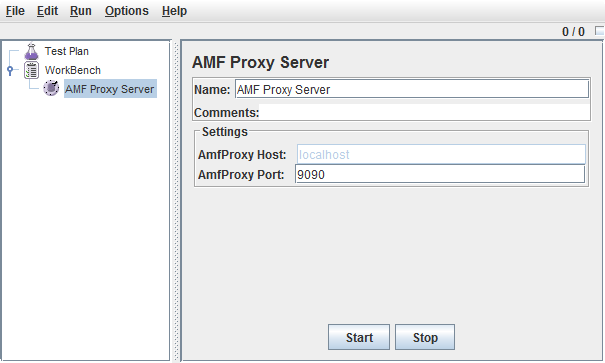
\includegraphics[height=60mm, width=80mm]{fig/development/proxySettings.png}}
\caption{Настройка прокси-сервера}
\label{ris:proxySettings.png}
\end{figure}

В поле AmfProxy Port необходимо указать номер порта, который будет слушать наш прокси сервер.
Если указать, например, 9090, то прокси-сервер будет запущен на localhost:9090.
Затем точно такие же настройки прокси-сервера устанавливаются в браузере, с помощью которого будет
производиться тестирование. Также стоит убедиться, что указанный Вами порт уже не занят другим приложением.

\subsection{Запись тестового сценария}

После того, как в AMF Proxy Server установлены все необходимые параметры, нажимается кнопка Start,
запускающая прокси-сервер.

\begin{figure}[h]
\center{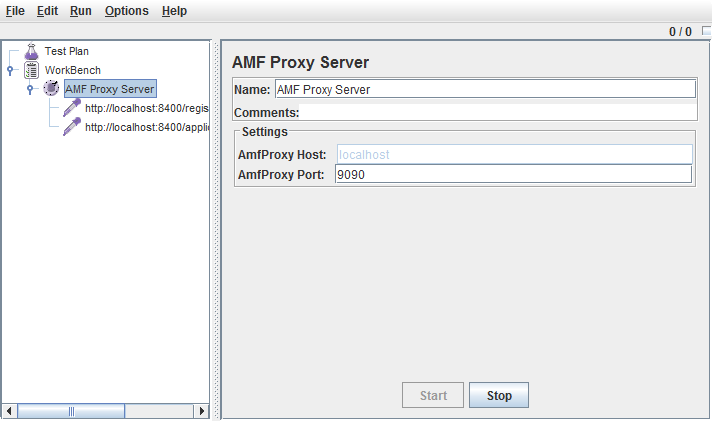
\includegraphics[height=60mm, width=80mm]{fig/development/proxyStart.png}}
\caption{Запуск прокси-сервера}
\label{ris:proxyStart.png}
\end{figure}

Затем тестируемое приложение открывается в браузере, для которого также
применены соответсвующие настройки прокси-сервера, и пользователь может выполнять с Flex приложением
необходимые операции, которые будут записываться AMF Proxy Server в виде элементов AMF RPC Sampler и в
дальнейшем могут быть перенесены в тест-план. Чтобы завершить запись тестовых запросов, необходимо
нажать кнопку Stop. После завершения записи тестов, все перехваченные запросы отображаются в дереве
элементов JMeter в качестве дочерних элементов AMF Proxy Server.

\subsection{Создание тест-плана}

Создание тест-плана в JMeter осуществляется следующим образом.
В первую очередь добавляется группа потоков - Thread Group (Test Plan > Threads (Users) > Thread Group).

\begin{figure}[h]
\center{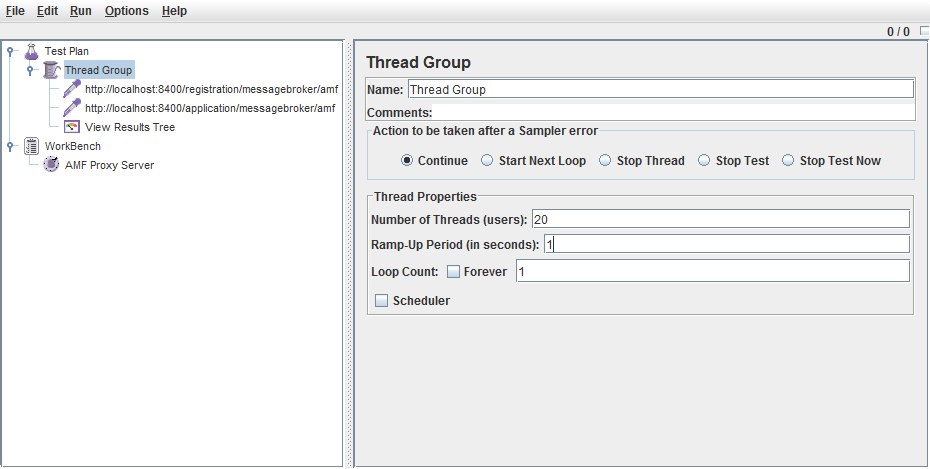
\includegraphics[height=60mm, width=80mm]{fig/development/testplan.png}}
\caption{Создание тест-плана}
\label{ris:testplan.png}
\end{figure}

Этот элемент является ключевым в тест-плане JMeter, именно его функционал отвечает за реализацию
нагрузочного тестирования --- многопоточного запуска последовательности тестовых шагов.
В данном элементе задается следующее:

\begin{enumerate}
\item Действия, которые будут производиться в случае, если в тест выполняется с ошибкой
(Action to be taken after a Sampler error);
\item Число потоков, в которое будут запускаться шаги тест-плана (Number of Threads);
\item Интервал, в течение которого будет запущено указанное в предыдущем параметре
число потоков (Ramp-Up Period);
\item Число повторений набора тестов (Loop Count);
\item Расписание запуска тестов (Scheduler).
\end{enumerate}

Затем в Thread Group в качестве дочерних элементов добавляются шаги тестов, которые
будут запускаться с указанными характеристиками. В нашем случае мы переносим элементы
AMF RPC Sampler, записанные с помощью прокси.
Помимо этого следует добавить визуалайзер результатов, чтобы иметь возможность
отслеживать ход тестового сценария (Thread Group > Add > Listener ).
JMeter предлагает большой выбор таких элементов, для примера будем использовать View Results Tree.
После того как план сформирован, он может быть сохранён. (File > Save Test Plan As...)

\subsection{Запуск тестов}

Чтобы запустить содержимое элемента Test Plan, необходимо выбрать в основном меню Run > Start.
После заврешения прогона тестов результаты их выполнения можно наблюдать в View Results Tree.

\section{Методика тестирования}


